\section{Belt drive simulation}\label{sec:beltdrive}
In this section, we investigate the dynamics of a belt drive system featuring two pulleys, $P_1$ and $P_2$, both with identical radius and inertia, as illustrated in \fig{fig:ESR8_BeltDrive}. The numerical modeling of this system relies on the Absolute Nodal Coordinate Formulation (ANCF), with the pulleys simulated as rigid bodies and the belt-pulley contact modeled as per \cite{Ntarladima2023}.
The repository for the code related to this section is located at:
\bi
  \item[] \url{https://github.com/THREAD-2-3/beltDriveSimulation}
\ei

\subsection{Description of belt drive simulation}
The examined belt drive has two pulleys $P_1$ and $P_2$ with identical radius and inertia, see the geometrical setup in \fig{fig:ESR8_BeltDrive}.
%
The numerical modeling of the belt is based on the Absolute Nodal Coordinate Formulation, \cite{Gerstmayr2008}. The pulleys are simulated as rigid bodies while the contact between the belt and pulleys is modeled as described in \cite{Ntarladima2023}.


%
This numerical example is similar to the one developed in \cite{Pechstein2013} with some modifications which attempt to eliminate the vibrations at the beginning of the simulation and allow the system to reach the steady state. The angular velocity of pulley $P_1$ is prescribed using an algebraic constraint, while some resistance torque over time is added to pulley $P_2$, see the description hereafter.
%++++++++++++++++++++++++++++++++++++++++++++++++++++++++++++++++++++++
\begin{figure}[tbph]
    \centering
    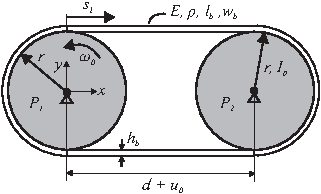
\includegraphics[width=0.55\textwidth]{figures/ESR8_beltPechstein.pdf}
    \caption{Belt drive with two pulleys, displaced from the initial position by $u_0$.}
    \label{fig:ESR8_BeltDrive}
\end{figure}
%++++++++++++++++++++++++++++++++++++++++++++++++++++++++++++++++++++++
\begin{table}[tbph]
    \caption{Main parameters for the belt drive.} \label{tab_beltdriveParameters}
    \centering
    %\begin{tabular}{@{}lrlp{0.4\textwidth}@{}} \toprule
    \begin{tabular}{c|c|c|c|c} \hline
        Par. & Value & Units & Description & variable name in code\\ \hline 
        $r$ & 
            $0.09995$ & \si{\meter} &
            pulley radius & \pythoninline{radiusPulley} \\
        $d$ & 
            $0.1 \pi$ & \si{\meter} &
            distance between two pulleys & \pythoninline{distancePulleys} \\
        $h_b$ & 
            $0.0001$ & \si{\meter} & 
            belt height &\pythoninline{hc} \\
        $w_b$ & 
            $0.08$ & \si{\meter}  & 
            belt width &\pythoninline{b} \\
        $\bar l_b$ & 
            $0.38 \pi$ &  \si{\meter} &  stress-free belt length & (computed)
            \\
        $l_b$ & 
            $0.4 \pi$ &  \si{\meter} &
            initial, deformed belt length & (computed)\\
        $\varepsilon_{ref}$ & 
            $-0.05$ &  - &
            added reference axial strain %of the belt
             & \pythoninline{preStretch}\\% (causing pre-tension)\\
%        $u_0$ & 
%            $0.$ & \si{\meter} &
%            horizontal displacement (used only in original model \cite{Pechstein2013})\\
 %       $E$ & 
%            $10^7$ & \si{\newton \per \meter \squared} &
 %           Young's modulus \\
        $EA$ & 
            $8000$ & \si{\newton \meter} &
            axial stiffness & \pythoninline{EA} \\ 
        $EI$ & 
            $\frac{4}{3} \cdot 10^{-3} $ & \si{\newton \meter \squared} &
            bending stiffness & \pythoninline{EI}\\             
        $\rho$ & 
            $1036$ & \si{\kilogram \per \meter ^3}&
            beam density & \pythoninline{rhoA}\\
        $dEA$ & 
            $1$ & \si{\newton \per {\meter \second}\squared} &
            strain proportional damping & \pythoninline{dEA} \\ 
        $\omega_{P1}$ & 
            $12$ & rad \si{\per \second} & 
            angular velocity of $P_1$ & \pythoninline{omegaFinal}\\
        $d_{P2}$ & 
            $2$ & \si{\newton \meter \per {\second}} &
            %angular velocity proportional 
            damping at $P_2$ & \pythoninline{rotationDampingWheels}\\ 
        $t_0$ & 
            $0.05$ & \si{\second} & 
            driving start time & \pythoninline{tAccStart}  \\
        $t_1$ & 
            $0.60$ & \si{\second} & 
            driving end time & \pythoninline{tAccEnd} \\
        $t_{\tau 0}$ & 
            $1.0$ & \si{\second} & 
            torque $\tau_{P2}$ starts
            %raised at pulley $P_2$  
            &\pythoninline{tTorqueStart} \\
        $t_{\tau 1}$ & 
            $1.5$ & \si{\second} & 
            torque $\tau_{P2}$
            % at pulley $P_2$ 
            reaches nominal value & \pythoninline{tTorqueEnd}\\
        $I_p$ & 
            $0.25$ & \si{\kilo\gram \per \meter \squared} & 
            moment of inertia of  pulleys & \pythoninline{wheelInertia} \\
        %$\mu$ & 
            %$0.5$ & - & 
            %friction coefficient \\
        %$c_c$ & 
            %$4\cdot 10^9$ & \si{\newton \per \meter ^3} & 
            %contact stiffness \\
        $g$ & 9.81 & \si{\meter \per \second \squared} & gravity & \pythoninline{gVec}
 \\ \hline
        %\bottomrule
    \end{tabular}
\end{table}
%++++++++++++++++++++++++++++++++++++++++++++++++++++++++++++++++++++++
%++++++++++++++++++++++++++++++++++++++++++++++++++++++++++++++++++++++
The belt is modeled as a Bernoulli-Euler beam with bending stiffness $EI$, axial stiffness $EA$, rectangular cross-section with height $h_b$ and width $w_b$, as well as stretch proportional damping, density, and further parameters given in \mytab{tab_beltdriveParameters}.
A linearly increasing angular velocity is prescribed to pulley $P_1$ between $t_0$ and $t_1$:
\be \label{eq:ESR8_torqueP2}
  \omega_{P1}(t) = \begin{cases} 0\,\frac{\si{\radian}}{\si{\second}},\quad \quad \quad \quad \quad \quad \quad \quad \quad \quad\,\;\;\mathrm{if} \quad t < t_{0} \\
                  \omega_{P1} \frac{t-t_{0}}{t_{0}-t_{1}}\quad \quad  \quad \quad \quad \quad \quad \quad \quad \;\mathrm{if} \quad t_{0} < t < t_{1} \\ 
                  \omega_{P1} \, \quad \quad \quad \quad \quad \quad \quad \quad \quad \quad \quad \mathrm{else} \, .
                 \end{cases}
\ee
% by varying the angular velocity between $0$ and $\omega_{P1}$. Hereafter, a constant angular velocity $\omega_{P1}$ is prescribed to pulley $P_1$. 


A torque proportional to the angular velocity is applied to the pulley $P_2$ which represents the damping of rotational motion:
\be \label{eq:ESR8_torqueP2}
  \tau_{P2}(t) = \begin{cases} 0\,\mathrm{Nm}, \quad \quad \quad \quad \quad \quad \quad \quad \quad \quad \quad \quad \,\;\;\mathrm{if} \quad t < 1 \\
                  25\left(0.5-0.5\cdot \cos\left( 2 (t-1) \pi \right) \right)\mathrm{Nm} \quad \mathrm{if} \quad 1 < t < 1.5 \\ 
                  25\,\mathrm{Nm} \quad \quad \quad \quad \quad \quad \quad \quad \quad \quad \quad \quad \,\,\;\mathrm{else} \, .
                 \end{cases}
\ee

As compared to \cite{Pechstein2013}, we use a much smaller belt height $h_b$ to exclude bending effects and a higher pre-tension (due to pre-stretch), while keeping the axial stiffness $EA$ the same. Furthermore, the bending stiffness is lowered by a factor of $50$, which reduces bending effects, as it would lead to significant deviations from an analytical solution otherwise.
The support of pulley $P_1$ is not displaced during the first $0.05\,$s of the simulation, but the pre-stretch $\varepsilon_{ref}$ is applied before running a static computation, which defines a static equilibrium for the dynamic simulation hereafter.
The contact stiffness has been increased by a factor of $40$ and a tangential stiffness (bristle) model has been included to retrieve highly accurate contact behavior. % To investigate steady-state behaviour, the belt drive is first accelerated up to nominal angular velocity $\omega_{P1}$:

% and in the time range $t=[1\,\mathrm{s}, \; 1.5\,\mathrm{s}]$ an additional torque of $25\,$Nm is added to pulley $P_2$, see \eq{eq:ESR8_torqueP2}. 
%At $t=1\,$s an additional torque is added and raised until $t=1.5\,$s to a constant torque of $25\,$Nm by means of the function


